\chapter{The image reconstruction problem}

%Reconstructing accurately the desired domain is a complicated mathematical problem that is actively being researched since the invention of CT. However, nowadays the FDK algorithm is the most widely used algorithm, and only until very recently [CITE] it has been the only algorithm available in any commercial medical reconstruction device. While using FDK is advantageous in some cases, often the algorithm behaves poorly, specially when errors arise in the data, or the amount of data is limited. This is because FDK is based on a derivation of straight path integrals in continuous spaces. Reality is far from straight path integrals, as due to X-ray physics photons do not behave linearly. Photons from CT machines are polychromatic, and human tissue is behaves non-linearly in respect to X-ray energy. Additionally, Compton scattering is a common effect, where the photons get reflected in different angles dependent on their energy. Apart from physics, electronic noise is always present in detector technology being the only feasible way of avoiding it longer exposition times, harmful to live tissue. Limited data can additionally harm the image reconstruction, as CT has generally less detector data than the amount of  voxels are desired to reconstruct. All these effects make CT image reconstruction a challenging problem and have strong effect in the behaviour of FDK. As an alternative to FDK, iterative algebraic reconstruction algorithms try to minimize the error by updating the image continuously and comparing it to the measured data. These algorithms have been shown to improve reconstruction quality when the data is noisy and/or limited. Additionally, as they are an algebraic tool, they allow careful tuning of the mathematics on there, enabling them to be tuned to correct any chose effect. 

This chapter tries to explain the mathematics behind CT reconstruction, the FDK algorithm and iterative reconstruction algorithms. After the formal proposition of the mathematical problem of integrating over straight lines,the FDK algorithm is introduced. Then, the alternative proposal of the iterative algebraic methods is shown, followed by a wide variety of different algorithms that can be used to solve the algebraic problem. These include gradient descend techniques, Krylov subspace methods, statistical approaches and compressed sensing techniques. Finally, a discussion of the challenges that arise from the use iterative algorithms are described.  

\section{Geometry of CBCT}

\section{FDK}

\section{Iterative reconstruction algorithms}
Nowadays the FDK algorithm is the most widely used algorithm, and only until very recently [CITE] it has been the only algorithm available in any commercial medical or industrial CT device. While using FDK is advantageous in some cases, often the algorithm behaves poorly, specially when errors arise in the data, or the amount of data is limited. This is because FDK is based on an analytical approximation of straight path integrals in continuous spaces. Reality is far from straight path integrals, as due to X-ray physics photons do not behave linearly. Photons from CT machines are polychromatic, and human tissue is behaves non-linearly in respect to X-ray energy. Additionally, Compton scattering is a common effect, where the photons get reflected in different angles dependent on their energy. Apart from photon physics related errors, electronic noise is always present in detector technology being the only feasible way of avoiding it longer exposition times, harmful to live tissue. Limited data can additionally harm the image reconstruction, as CT has generally less detector data than the amount of  voxels are desired to reconstruct. All these effects make CT image reconstruction a challenging problem and have strong effect in the behaviour of FDK. As an alternative to FDK, iterative algebraic reconstruction algorithms try to minimize a functional by updating the image continuously and comparing it to the measured data. These algorithms have been shown to improve reconstruction quality when the data is noisy and/or limited. Additionally, as they are an algebraic tool, they allow careful tuning of the mathematics, enabling them to change their behaviour.

Iterative algorithms in CT generally reffer to those algorithms that, as the name says, iterate, but solve the linearized model 
\begin{equation}
Ax=b+\tilde{e} \label{eq:linearized model}
\end{equation}
on where $x\in \mathbb{R}^{N_{voxels}}$ is a vector representing the lexicographically ordered voxels of the 3D image, $b\in \mathbb{R}^{N_{pixels}} $ a vector of the detector measured pixels. $A$ is the linearized model matrix, a matrix that describes the behaviour of the CT system. Each row of the matrix $A$ is describes the behaviour of the X-rays that affect each single pixel in the detector. However, this matrix is so big that in practize its explicit form is impossible to store, and the matrix product operations $Ax$ (or projection) and $A^Tb$ are implemented instead. The next chapter goes into a bit more detail on how to operate with matrix $A$ and its limitations. Errors from measurement are inevitable in any application, and there are linearization errors, as no model is perfect. In equation \ref{eq:linearized model}, $\tilde{e}$ represents all those errors.

As an exact solution for $x$ can not be found, the problem in equation \ref{eq:linearized model} is minimized as
\begin{equation}
\hat{x}=\argmin_x \lVert Ax-b\rVert^2+R(x),\label{eq:THE equation}
\end{equation}
on where $R(x)$ is an optional regularization function. This minimization function has been widely studied in mathematics and there are multiple algorithms that can solve it. However not all algorithms that solve the equation can be used in CT reconstruction, due to the nature of the $A$ matrix, as it is very big (approximately $10^8\times 10^8$ in a standard medical image) and very sparse (approximately $0.0017\%$ of sparsity in a standard medical image). This makes the matrix severely ill-conditioned and impossible to store in memory. Additionally, often the CT problem can be underdetermined, making the problem ill-posed and further constraining the possible algorithms that can be used. That said, a wide variety of algorithm have been proposed to solve the CT algebraic problem and new ones are still being published. This section discusses a few of the available and most common algorithms that have been studied in this work.


\subsection{Algebraic Reconstruction Techniques}

Arguably the most well known iterative algorithm is the method known as the algebraic reconstruction technique (ART)\cite{K-1937}, known as the Kaczmarz method outside the CT imaging field. The ART algorithm, for matrix elements $a_{ij}\in R$ is defined as
\begin{equation}
x^{n+1}=x^n+\frac{b_i-\langle a_i,x^n\rangle}{\lVert{a_i}\rVert^2}a_i^T,
\end{equation}
where $a_i$ is the $i$-th row of matrix $A$ and $\langle \,, \rangle$ denotes the inner product. The ART method projects the image into the hyperplane described by the equation in row $i$. Generally the method includes a relaxation parameter $\lambda_n$ that controls the update size, and that decreases with the iteration number. This generally avoids the cyclical convergence that the method describes when the solution is not unique (the intersection of the hyperplanes is not a single point). By relaxing the update step, the algorithm converges to a single point. Generally the algorithm is also run with some inequality constrains, the most common one being a positivity constrain for $x$, as negative values are not physically possible.

Studies on the convergence of the ART algorithm show\cite{241889} that randomly choosing the order of the rows in each iteration ($n$) increase the convergence rate, even more if the probabilities of picking rows are different than one (different methods propose different probabilities)\cite{strohmer2009randomized}\cite{liu2016accelerated}. 

However, the ART method has a major disadvantage: the image $x^{n+1}$ needs to be updated $i$ times each iteration. In current CT applications, and specifically in CBCT, the amount of rows in the matrix i.e. the total amount of independent pixel measurements in the detector is a massive number. Following the same definition of standard medical image size from the thesis, a $512\times512$ detector, with 360 projection means that the amount of rows is in the order of $10^8$. In order to update the image less, the Simultaneous Iterative Reconstruction Technique (SIRT)\cite{SIRT} can be used, a method that is very similar to Cimmino's method, that updates the image using simultaneously (instead of sequentially) all data in the measurement $b$, thus each iteration is a single update. While SIRT generally solves the problem of the high amount of updates in ART, it suffers from a very slow convergence in comparison, and will generally plateau in a solution that is not as good as what ART provides. The SIRT algorithm can be described in matrix form as
\begin{equation}
x^{n+1}=x^n+\lambda_n V A^T W^{-1}\left(b-Ax\right) \label{eq:SIRT}
\end{equation}
where $V=1/\text{diag}\bigl({\sum_j a_{ij}}\bigr)$ and  $W=\text{diag}\bigl({\sum_i a_{ij}}\bigr)$.

However, middle ground has also been proposed. Kak and Andersen proposed\cite{SART} the Simultaneous Algebraic Reconstruction Technique (SART) on where the image is updated using simultaneously all data from each X-ray projection, but still updating the image multiple times per iteration. Finally, the update can also be done using block-based methods, or Oriented Subsets (OS) with a variety of methods generally described as OS-SART\cite{OS_SART} methods.

 Similarly as with ART, the order of the subsets in both OS-SART and SART have influence in the convergence, with a lower impact than in ART. In this work an three methods have been implemented, a completely ordered method, a randomized ordered method with full sampling (i.e. all projections are ensured to be used once and only once per iteration) and an angular distance based one. This last one orders the subsets by selecting the next one as the subset with largest angular distance from the ones already used. The heuristic rationale is that the projections at larger angular distance update the image by a bigger step than projections angularly near. In all further result in this thesis, the default ordering is random, unless otherwise explicitly stated.
 
 %% SHOW CONVERGENCE WITH DIFFERENT ORDERING



\subsubsection{Relaxation parameter $\lambda$}

As previously mentioned, changing the relaxation parameter per iteration can be of advantage, by avoiding cyclical convergence and often by increasing the general convergence rate. On of the commonly used methods for the reduction of lambda is simply reducing it by a reduction factor each iteration as
\begin{equation}
\lambda_{n+1}=\lambda_n*r_\lambda
\end{equation}
where $r_\lambda$ is some value close to one, such as $r_\lambda=0.99$ or $r_\lambda=0.999$. However this method, while useful to avoid cyclical convergence in ART methods, is of less use in simultaneous methods, as it generally slows the convergence rate.% Alternatively, convergence studies for SART/OS-SART/SIRT algorithms have shown\cite{jiang2003convergence} that an update of the relaxation parameter in the form of
%\begin{equation}
%\lambda_{n+1}=\frac{\lambda_0}{1+n^\alpha}
%\end{equation}
%where $\lambda_0$ is an initial value of the relaxation parameter (usually 1) and $0<%\alpha\leq 1$. this can improve the convergence of the algorithms. 

It is worth noticing that this family of algorithms is very closely related to the well known gradient descend methods, as the gradient of equation \ref{eq:THE equation} is  proportional to $A^T(Ax-b)$, or in other words $V=I$ and $W=I$ in equation \ref{eq:SIRT}. The gradient descend methods have been widely studied in the past years\cite{sutskever2013importance}\cite{DBLP:journals/corr/Ruder16}, as the Neural Networks community tries to find faster converging methods to train the nets they research. Among other methods proposed, Nesterov proposed an accelerated version of the gradient descend\cite{nesterov1983method}, that obtains a rate of convergence of $1/n^2$. The proposed update   updates the result image in each iteration by pushing it in the current update and previous update direction combined. Nesterovs Accelerated Gradient (NAG) defines
\begin{align}
\lambda_{n+1}&=\frac{1+\sqrt{1+4\lambda_{n}^2}}{2}\\
\gamma_n&=\frac{1-\lambda_n}{\lambda_{n+1}}\\
y^{n+1}&=x^{n}-\frac{1}{\beta}\nabla f(x^n)\label{eq:Nesterov update 1}\\ 
x^{n+1}&=(1-\gamma_n)y^{n+1}+\gamma y^n
\end{align}
with $\lambda_0=1$ and $\beta$ being the Lipschitz smoothness of the function $f$. The line in equation \ref{eq:Nesterov update 1} can be replaced by the SART/OS-SART/SIRT update on equation \ref{eq:SIRT} to obtain an accelerated convergence rate. Some experimental results on the convergence of the algorithms can be found in Chapter 5.
\subsection{Conjugate Gradient Least Squares}

The conjugate gradient for the least squares problems (CGLS) 
\subsection{Statistical inversion}
\subsection{Total variation minimization with POCS}

Sometimes solving a regularized problem may result in a better final image than just trying to solve the data constrain with the model. This is especially useful in more ill-conditioned problems, such as when the data is very noisy (thus the model does not fit the data with accuracy) or when few projections are available (the system is more under-determined). In these cases, regularisation can add a user constrain in the image domain that pushes the algorithm towards an specific solution among all the multiple possibilities. While a variety of regularization techniques and norms exist, the most suitable for CT imaging is the total variation (TV) norm.

The total variation norm is defined as the sum of the 2-norms of the directional gradients of the variable,

\begin{equation}
\lVert x \rVert_\text{TV}=\sum_n\left\lVert \sum_\alpha\partial_\alpha x_n \right\rVert_2.
\end{equation}

Applied to CT imaging, the total variation norm is the sum of the total change occurred in the image. An image with less total variation would be an image that would have less change, or more flat, same valued regions. Regularizing with the TV norm as a minimization term will yield an image that is piecewise smooth and it happens that most of the objects imaged in CT scanners are piecewise smooth in linear attenuation, even more in medical CT imaging. 

However, solving the minimization problem in equation XX is not trivial with the TV regularization. One of the first robust algorithm is the so called Adaptive Steepest Descend, Projection Onto Convex Subsets, or ASD-POCS algorithm\cite{ASD_POCS}. This algorithm not only minimizes the data constrain with TV regularization but also adaptively controls the TV minimization update, in order to adapt its strength according to the data constrain update. Several adaptations and improvements of this algorithm have been proposed in the literature[CITES], all based in the same mathematical basis.  


\subsubsection{ASD-POCS}

The previous algorithms discussed in this chapter where unconstrained minimization methods. While the TV minimization problem can be solved similarly (see section \ref{sec:SART-TV}) formalizing the algorithm as a non-linear constrained minimization adds an advantage in the case where there system is under-determined. In an unconstrained problem such as in equation XX, the balance between the data constrain and the regularization constrain can be tuned via a hyperparameter, but in the case of an under-determined system, multiple solutions for the data fidelity term may exist. By reformulating it as it is shown in the rest of this section, the image with the same data fidelity 2-norm but the lowest TV norm can be chosen.

The minimization will yield an image $\vec{x}^*$ that minimizes 

\begin{equation}
\vec{x}^*= \argmin_x \lVert \vec{x} \rVert_\text{TV}
\end{equation}
subject to 
\begin{align}
\lVert A\cdot \vec{x}-\vec{b}\rVert &\leq \epsilon,\label{eq:nl-datafid}\\
\vec{x}&\geq 0.
\end{align}

As previously described in this chapter, the data fidelity on equation \ref{eq:nl-datafid} while desired to be zero, it will never reach to zero, due to inconsistencies in the data, model, noise, etcetera. Thus, in this algorithm it is introduced as a inequality constrain, instead of as the minimization problem itself. This introduces the parameter $\epsilon$ in the algorithm, the maximum 2-norm allowed for the data inconsistency. The problem in hand is now non-linear, due to the constrains, but convex.

The conditions for a constrained minimization to find the optimal solution can be obtained by satisfying the Karush Kuhn-Tucker conditions (a generalization of the Lagrange multiplies for inequality constrains). First, the Lagrangian for the current problems needs to be defined, as

\begin{equation}
\textbf{L}=\lVert \vec{x} \rVert_\text{TV}+\lambda_0\cdot(\lVert A\cdot \vec{x}-\vec{b}\rVert^2 - \epsilon^2)-\vec{\lambda}\cdot\vec{x},\label{eq:Lagrangian}
\end{equation}
where $\vec{\lambda}$ is a vector of the same size as the image, but $\lambda_0$ is a single value. Two inequality constrains are imposed to the Lagrange multipliers, namely non-negativity
\begin{equation}
\lambda_i \geq 0,
\end{equation}
and complementarity 
\begin{equation}
h_i(\vec{x}) \lambda_i = 0,
\end{equation}
where $i=0,1,..., N_{pixels}$, and $h_i$ is an alternative form of the inequality constrains as
\begin{align}
h_0(\vec{x}) &=\lVert A\cdot \vec{x}-\vec{b}\rVert^2 - \epsilon^2 \leq 0&\\
h_i(\vec{x}) &= -x_i \leq 0 & i \in [1, N_{pixels}]
\end{align}

Thus, only when the inequalities are violated does $h_i$ turns non-zero, and with the complementarity condition, does the corresponding $\lambda_i$ turns zero. A solution can be found for $\vec{x}$ when the gradient of the Lagrangian is zero, and if the differential operator is defined as

\begin{equation}
\nabla_{\vec{x}}Q(\vec{x})=\sum_i {\partial_{x_i}}Q(\vec{x}) \vec{\delta}_i
\end{equation}
where $\vec{\delta}_i$ is the Kronecker delta. The gradient of the Lagrangian can be then written as
\begin{align}
\nabla_{\vec{x}}\textbf{L}&=\nabla_{\vec{x}}\lVert \vec{x} \rVert_\text{TV}+\lambda_0\nabla_{\vec{x}}h_0(\vec{x})+\sum_{i=1\textit{•}}^{N_{pixels}}\lambda_i\nabla_{\vec{x}}h_i(\vec{x})=0 \notag \\
&=\nabla_{\vec{x}}\lVert \vec{x} \rVert_\text{TV}+2\lambda_0 A^T\cdot(A\cdot\vec{x}-\vec{b})-\vec{\lambda}=0 \label{eq:KKT}
\end{align}

Further simplification can be applied to equation \ref{eq:KKT}. As the non-negativity constrains are only active in zero valued voxels, the Lagrange multipliers are zero for strictly positive voxels. Thus, by adding an indicator function
\begin{equation}
\vec{x}_{indic}=
\begin{cases}
1 & \vec{x} \neq 0 \\
0 & \vec{x} = 0 
\end{cases}
\end{equation}
the Lagrangian gradient can be shortened to
\begin{equation}
\nabla_{\vec{x}}\textbf{L}=\text{diag}(\vec{x}_{indic})\left(\nabla_{\vec{x}}\lVert \vec{x} \rVert_\text{TV}+\lambda_0\nabla_{\vec{x}}h_0(\vec{x})\right)=0 .\label{eq:KKT2}
\end{equation}
Separating this new equation into two vectors,
\begin{align}
\vec{d}_{\text{TV}}&=\text{diag}(\vec{x}_{indic})\left(\nabla_{\vec{x}}\lVert \vec{x} \rVert_\text{TV}\right)\notag\\ 
\vec{d}_{\text{data}}&=\text{diag}(\vec{x}_{indic})\left(\nabla_{\vec{x}}h_0(\vec{x})\right)
\label{eq:KKTvectors}
\end{align}
brings to the Karush Kuhn-Tucker conditions: $\vec{x}$ will be an optimal condition if $\vec{d}_{\text{TV}}$ and $\vec{d}_{\text{data}}$ are pointing in exactly the opposite direction. In practice the algorithm will only check if the vectors are pulling in opposite direction (by computing the dot product) and that the inequality constrains are satisfied. By checking the direction of the vectors the algorithm ensures that even if the data constrain is satisfied, only the optimal solution regarding both TV norm and data fidelity is chosen.


\begin{figure}[H]
\begin{center}

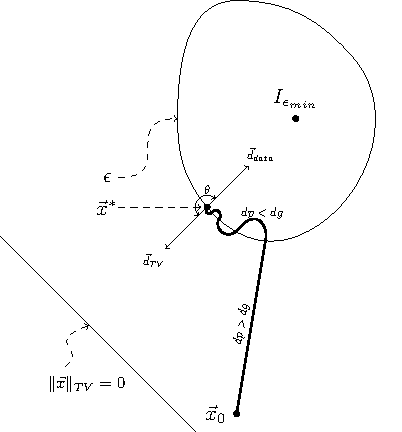
\includegraphics[scale=1.2]{RecAlgorithms/POCS.pdf} 
\end{center}

\caption[Diagram of the POCS algorithm]{\label{fig:POCSAlgo} Conceptual diagram of the ASD-POCS algorithm path to the solution.} 
\end{figure}


Figure \ref{fig:POCSAlgo} shows a conceptual diagram of the ASD-POCS algorithm. There is an area around the image with minimum data constrain, $I_{\epsilon_{min}}$. The solution $\vec{x}^*$ generally lies on the boundary of the area with the user specified $\epsilon$. From an initial image $\vec{x}_0$, the algorithm walks towards the area of acceptable $\epsilon$ more strongly than towards the area of minimum TV, as the step sizes of the vectors $\vec{d}_{\text{TV}}$ and $\vec{d}_{\text{data}}$, $dp$ and $dg$ respectively, are adaptively controlled to be $dp>dg$. Once the image is within acceptable 2 norm, then the step size is changed in order to have stronger $\vec{d}_{\text{TV}}$ ($dp<dg$). The optimal solution can be found when both vectors point in opposing direction, or in other words, when the angle between them is 180\ degrees, or the cosine of it is -1,

\begin{equation}
\cos \theta = \frac{\vec{d}_{\text{TV}} \cdot \vec{d}_{\text{data}}}{\lVert\vec{d}_{\text{TV}}\rVert \lVert\vec{d}_{\text{data}}\rVert }.
\end{equation}


The pseudocode for the algorithm can be seen in algorithm \ref{alg:ASD-POCS}. The algorithm is essentially solving the two vector in equation \ref{eq:KKTvectors}, the data vector in lines [5-8] and the TV vector in lines [18-22]. Line [9] enforces the positivity constrain. In the algorithm, $dtv$ is initialized according to $\alpha$, an user specified   TV hyperparameter for TV, together with $dp$, the step size performed by the data constrain. After the TV minimization is performed, the step size of the TV vector is rechecked. If the TV minimization step is too big (bigger than the data step size), and the desired $\epsilon$ is still not achieved, the step size is reduced further. This method of adaptively setting the step size of the TV iteration relating to the data step size is what ensures the optimal condition is achieved. Finally, the stopping criteria relies in either achieving the desired $\epsilon$ with with a desired $\cos \theta$, or stopping due to reaching a maximum amount of iterations ($\beta$ decreases with iteration number). In the original proposition of the ASD-POCS algorithm (and shown here), the data constrain is solved using SART, however any other algorithm solving the same minimization problem can be used here (e.g. CGLS or OS-SART).


The algorithm has 7 parameters that need to be set up: $\beta$ and $\beta_{red}$ are the initial value and reduction ratio of the SART hyperparameter, similarly $\alpha$ and $\alpha_{red}$ serve as hyperparameter and reduction ratio for the TV minimization. $r_{max}$ controls the maximum allowed ratio of change between the data minimization and the TV minimization, in order to adapt the step sizes. The number of iterations the TV minimization performs per iteration of the data minimization is defined as $n_{TV}$. Finally, the allowed data error is $\epsilon$, as described before. The initial values of the variables in the algorithm are a key factor on its convergence. Empirical tests show that wrong parametrization of the algorithm can lead to severely noisy reconstructions. An study of the sensitivity of these parameters to changes has been performed by Lohvithee \emph{et al}\cite{Vee}. The study shows that some parameters can be safely set up to a static value regardless of the data, such as the data hyperparameters, but that $\epsilon$, $n_{TV}$ and $\alpha$ are critical parameters to tune in order to get an usable reconstruction, and they are heavily data dependant. While some algorithms have successfully replaced the initial set of $\alpha$ by some data based heuristics [CITE PCSD]\footnote{These algorithms, namely PCSD and Aw-PCSD, are also available in TIGRE, by Manasavee Lohvithee.} to the best of the authors knowledge there is no mathematical proposal for setting these parameters. The biggest drawback of this method is that several reconstructions may be needed to find the best parameters for an specific application.

Note that this minimization approach, while used for TV minimization in the original article, can be used for a variety of different minimization functions. For example, the TV minimization step could be replaced by a prior image minimization[CITE PICS], or any other convex minimization function. Similarly, the data minimization step can be replaced by any other minimization algorithm, as long as it minimizes the problem in equation XX
\begin{algorithm}

\caption{ASD-POCS
\label{alg:ASD-POCS}}
\begin{algorithmic}[1]
\State{Set: $\beta, \beta_{red}, n_{TViter}, \alpha, \alpha_{red}, r_{max} $}
\State{$\vec{x}=0$};
\While{Stopping criteria not met}
\State $\vec{x}_{prev}=\vec{x}$
\For {$n_{angles}$}
\State  $\vec{x}=\vec{x}+\beta V A^T W^{-1} (\vec{b}-A\vec{x})$
\Comment SART update
\EndFor
\State $\beta=\beta*\beta_{red}$
\State $\vec{x}=\max(0,\vec{x})$
\Comment Enforce positivity
\State $\vec{x}_{out}=\vec{x}$

\State $\epsilon_{now}=\lVert A\vec{x}-\vec{b}\rVert$
\Comment Current $\epsilon$
\State $dp=\lVert\vec{x}-\vec{x}_{prev}\rVert$
\Comment Change in $\vec{d}_{\text{data}}$

\If {first iteration}
\State{$dtv=\alpha*dp$}
\Comment Initialize TV hyperparameter
\EndIf

\State $\vec{x}_{prev}=\vec{x}$
\State
\For {$n_{TViter}$}
\Comment TV update
\State $\vec{dx}= \nabla_{\vec{x}} \lVert\vec x \rVert_{TV}$
\State $\hat{dx}=\vec{dx}/\lVert\vec{dx}\rVert$
\State $\vec{x}=\vec{x}-dtv\cdot\hat{dx}$
\EndFor
\State $dg=\lVert\vec{x}-\vec{x}_{prev}\rVert$
\Comment Change in $\vec{d}_{\text{TV}}$
\If{$dg>r_{max}*dp$  \textbf{and} $\epsilon_{now}>\epsilon$}
\State $dtv=dtv*\alpha_{red}$
\EndIf
\State
\Comment Check stopping criteria
\State $\cos\theta=\vec{dp}\cdot\vec{dg}/\lVert\vec{dp}\rVert\cdot\lVert\vec{dg}\rVert$
\If {($\cos\theta<-0.9$ \textbf{and} $\epsilon_{now}<\epsilon$) \textbf{or} $\beta<0.005$}
\State Stop
\EndIf
\EndWhile

\end{algorithmic}

\end{algorithm}


\FloatBarrier

\subsubsection{B-ASD-POCS-$\beta$}

Xue \textit{et al}[CITE] proposed a faster converging modification of the ASD-POCS algorithm by adding a relaxed Bregman iteration to the overall algorithm. The Bregman iteration updates the projection data with part of the remaining error, thus reducing the residual faster and reaching convergence faster. The top level pseudo-code of the B-ASD-POCS-$\beta$  can be seen in algorithm \ref{alg:B-ASD-POCS}.
%

\begin{algorithm}

\caption{B-ASD-POCS-$\beta$
\label{alg:B-ASD-POCS}}
\begin{algorithmic}[1]
\State{Set: $\beta, \beta_{red}, n_{TViter}, \alpha, \alpha_{red}, r_{max} $}
\State{$\beta$ update ratio:$c<1$}
\State{$\beta$ update period: $T$}
\State{$\vec{x}=0$};
\While{Stopping criteria not met}
\For{$n_{Bregman}$}
\State ASD-POCS algorithm
\EndFor
\State $\vec{b}=\vec{b}+\beta\cdot(\vec{b}^0-A\cdot\vec{x})$
\State Update $\beta=c\cdot\beta$ if current iteration is update period $T$ multiplier 
\EndWhile

\end{algorithmic}

\end{algorithm}

\FloatBarrier
\subsubsection{The gradient of the TV norm}

In order to minimize the TV norm via gradient descend, the gradient of the TV norm needs to be computed, $ \nabla_{\vec{x}} ||\vec x ||_{TV}$, being $\vec x$ the vectorized form of a N-dimensional image.

The main challenge wit the $ \nabla_{\vec{x}} ||\vec x ||_{TV}$ term is that $ ||\vec x ||_{TV}$ is not differentiable in the general case. However, in the CT case, $\vec{x}$ can be described as $x_{ijk}$, a regularly discretized mesh of directional indices $i,j,k$ of maximum value $i_{max},j_{max},k_{max}$. The gradient of $x$ has an additional Cartesian index $\alpha$:

\begin{align}
g^\alpha &=\left(\nabla x\right)^\alpha=\partial_\alpha x\\
g^\alpha_{ijk} & = \partial_\alpha x_{ijk}.
\end{align}

The TV norm can me then defined as sum of the 2-norms of the gradient of $x$, $g$, over the Cartesian coordinate, resulting in a scalar.

\begin{align}
\lVert x \rVert_\text{TV}=\sum\limits_{ijk} \sqrt{\sum\limits_\alpha \left(g^\alpha_{ijk}\right)^2}=\sum\limits_{ijk} \sqrt{\sum\limits_\alpha \left(\partial_\alpha x_{ijk}\right)^2},
\end{align}

This is the term that the total variation regularization algorithm minimizes with a gradient descend. In order to perform this, the gradient of this term with respect to $x$ is needed, now defined in a scalar field
\begin{equation}
 (\nabla_{\vec{x}} || x ||_{TV})_{ijk}.
\end{equation} 

This derivative can be expanded to a 3 component value for each $x_{ijk}$ as:
\begin{align}
\left(\nabla_x \lVert x \rVert_\text{TV}\right)_{ijk}&= \frac{\partial}{\partial x_{ijk}} \lVert x \rVert_\text{TV} = \partial_{x_{ijk}} \sum\limits_{i^\prime j^\prime k^\prime} \sqrt{\sum\limits_\alpha \left(\partial_\alpha x_{i^\prime j^\prime k^\prime}\right)^2}\nonumber
\\
&= \sum\limits_{i^\prime j^\prime k^\prime} \partial_{x_{ijk}}\sqrt{\sum\limits_\alpha \left(\partial_\alpha x_{i^\prime j^\prime k^\prime}\right)^2} \nonumber \\ 
&=\sum\limits_{i^\prime j^\prime k^\prime} \frac{\sum_\alpha\left(\partial_\alpha x_{i^\prime j^\prime k^\prime}\right) \partial_{x_{ijk}} \left(\partial_\alpha x_{i^\prime j^\prime k^\prime}\right)}{\sqrt{\sum\limits_\alpha \left(\partial_\alpha x_{i^\prime j^\prime k^\prime}\right)^2}}.\label{eq:gradientTVdisc}
\end{align}

This term now contains $\partial_\alpha$ derivatives, i.e. derivatives in the Cartesian coordinate system $[x,y,z]$. These are defined as

\begin{align}
\partial_x x_{i^\prime j^\prime k^\prime} &= \lim\limits_{h\to 0} \frac{x_{i^\prime+h,j^\prime,k^\prime}-x_{i^\prime, j^\prime, k^\prime}}{h} \nonumber \\
\partial_y x_{i^\prime j^\prime k^\prime} &= \lim\limits_{h\to 0} \frac{x_{i^\prime,j^\prime+h,k^\prime}-x_{i^\prime, j^\prime, k^\prime}}{h} \nonumber \\
\partial_z x_{i^\prime j^\prime k^\prime} &= \lim\limits_{h\to 0} \frac{x_{i^\prime,j^\prime,k^\prime+h}-x_{i^\prime, j^\prime, k^\prime}}{h}.\label{eq:derivativedef}
\end{align}

However, $x$ is discrete, thus the limit definition of the derivative can not be used to numerically compute it, but an approximation of it can. By setting $h=1$, equation \ref{eq:derivativedef} becomes the backward finite differences of the first order approximation of a derivative, a very computationally cheap operation. The derivative w.r.t. the Cartesian coordinate can be rewritten as

\begin{align}
\partial_\alpha x_{i^\prime j^\prime k^\prime}=\delta_{\alpha x} \left(x_{i^\prime,j^\prime,k^\prime}-x_{i^\prime-1, j^\prime, k^\prime}\right)&+ \delta_{\alpha y} \left(x_{i^\prime,j^\prime,k^\prime}-x_{i^\prime, j^\prime-1, k^\prime}\right)  \notag \\ &+ \delta_{\alpha z} \left(x_{i^\prime,j^\prime,k^\prime}-x_{i^\prime ,j^\prime, k^\prime-1}\right)\
\end{align}
 where $\delta_\alpha$ is a Kronecker delta for the Cartesian axis. The other partial derivative term that appears in equation \ref{eq:gradientTVdisc} is $\partial_{x_{ijk}} \left(\partial_\alpha x_{i^\prime j^\prime k^\prime}\right)$. As the derivative is w.r.t. $x_{ijk}$, each component of $x$ is an independent variable, thus $\partial_{x_{ijk}} \left(\partial_\alpha x_{i^\prime j^\prime k^\prime}\right)$ is zero everywhere but in indices $i=i^\prime \wedge j=j^\prime \wedge k=k^\prime$, where the derivative is 1. The term then becomes 
 \begin{align}
\partial_{x_{ijk}} \partial_x x_{i^\prime j^\prime k^\prime}&=\partial_{x_{ijk}}\left(x_{i^\prime,j^\prime,k^\prime}-x_{i^\prime-1, j^\prime, k^\prime}\right)=\delta_{i^\prime,i}\delta_{j^\prime,j}\delta_{k^\prime,k} - \delta_{i^\prime-1,i}\delta_{j^\prime,j}\delta_{k^\prime,k}\nonumber\\
&=\delta_{i^\prime,i}\delta_{j^\prime,j}\delta_{k^\prime,k} - \delta_{i^\prime,i+1}\delta_{j^\prime,j}\delta_{k^\prime,k}\nonumber\\
%
\partial_{x_{ijk}} \partial_y x_{i^\prime j^\prime k^\prime}&=\partial_{x_{ijk}} \left(x_{i^\prime,j^\prime,k^\prime}-x_{i^\prime, j^\prime-1, k^\prime}\right)=\delta_{i^\prime,i}\delta_{j^\prime,j}\delta_{k^\prime,k} - \delta_{i^\prime,i}\delta_{j^\prime-1,j}\delta_{k^\prime,k}\notag\\
&=\delta_{i^\prime,i}\delta_{j^\prime,j}\delta_{k^\prime,k} - \delta_{i^\prime,i}\delta_{j^\prime,j+1}\delta_{k^\prime,k}\nonumber\\
%
\partial_{x_{ijk}} \partial_z x_{i^\prime j^\prime k^\prime}&=\partial_{x_{ijk}} \left(x_{i^\prime,j^\prime,k^\prime}-f_{i^\prime, j^\prime, k^\prime-1}\right)=\delta_{i^\prime,i}\delta_{j^\prime,j}\delta_{k^\prime,k} - \delta_{i^\prime,i}\delta_{j^\prime,j}\delta_{k^\prime-1,k}\notag\\
&=\delta_{i^\prime,i}\delta_{j^\prime,j}\delta_{k^\prime,k} - \delta_{i^\prime,i}\delta_{j^\prime,j}\delta_{k^\prime,k+1}.
\end{align}

These terms are practically a selecting function for $i^\prime ,j^\prime ,k^\prime$ ,matching only in the indices $i,i+1,j,j+1,k,k+1$ in the sum of the right hand side of equation \ref{eq:gradientTVdisc}. However the indices are limited to $i^\prime \in [1,i_{max}]$, $j^\prime \in [1,j_{max}]$ and $k^\prime \in [1,k_{max}]$. As boundary conditions, Neumann boundary conditions are set to zero. To enforce that, a Kronecker deltas can be introduced for each index, $\left(1-\delta_{i,i_{max}}\right)$, with the same approach with the other indices.

Finally, substituting in equation \ref{eq:gradientTVdisc}, the gradient of the TV norm can be described as

\begin{align}
&\left(\nabla_x \lVert x \rVert_\text{TV}\right)_{ijk}=\sum\limits_{i^\prime j^\prime k^\prime} \frac{\sum_\alpha\left(\partial_\alpha x_{i^\prime j^\prime k^\prime}\right) \partial_{x_{ijk}} \left(\partial_\alpha x_{i^\prime j^\prime k^\prime}\right)}{\sqrt{\sum\limits_\alpha \left(\partial_\alpha x_{i^\prime j^\prime k^\prime}\right)^2}}\notag\\
&=\sum\limits_{i^\prime j^\prime k^\prime} \frac{\partial_x x_{i^\prime j^\prime k^\prime} \partial_{x_{ijk}} \left(\partial_x x_{i^\prime j^\prime k^\prime}\right) + \partial_y x_{i^\prime j^\prime k^\prime} \partial_{x_{ijk}} \left(\partial_y x_{i^\prime j^\prime k^\prime}\right) + \partial_z x_{i^\prime j^\prime k^\prime} \partial_{x_{ijk}} \left(\partial_z x_{i^\prime j^\prime k^\prime}\right)}{\sqrt{\sum\limits_\alpha \left(\partial_\alpha x_{i^\prime j^\prime k^\prime}\right)^2}}\notag \\
&=\frac{\partial_x x_{i,j,k}+\partial_y x_{i,j,k}+\partial_z x_{i,j,k}}{\sqrt{\sum\limits_\alpha \left(\partial_\alpha x_{i, j, k}\right)^2}}\notag \\
& - \frac{\left(1-\delta_{i,i_{max}}\right) \partial_z x_{i+1,j,k}}{\sqrt{\sum\limits_\alpha \left(\partial_\alpha x_{i+1, j, k}\right)^2}} - \frac{\left(1-\delta_{j,j_{max}}\right) \partial_y x_{i,j+1,k}}{\sqrt{\sum\limits_\alpha \left(\partial_\alpha x_{i, j+1, k}\right)^2}} - \frac{\left(1-\delta_{k,k_{max}}\right) \partial_z x_{i,j,k+1}}{\sqrt{\sum\limits_\alpha \left(\partial_\alpha x_{i, j, k+1}\right)^2}}.\label{eq:gradientTVnormNumerical}
\end{align}

Equation \ref{eq:gradientTVnormNumerical} is the numerical approximation of the gradient of the total variation norm, and describes scalar field of the same size of the image. The same approach can be used with central and forward differences to obtain a similar equation, however central differences may not correctly minimize the TV norm of the image. As central differences do not take into account the value of the current voxel $ijk$, a chequerboard pattern would have zero TV norm, and this is the opposite of the purpose of the algorithm, therefore only numerical approximations of derivatives that take immediately adjacent pixel values into account can be used (such as forward or backward finite differences).

\subsection{Total variation regularization via Rudin-Osher-Fatemi model} \label{sec:SART-TV}

A different minimization approach to POCS is the approach proposed by Jia \textit{et al}\cite{jia2011gpu}, that uses the Rudin-Osher-Fatemi (ROF) model for total variation minimization, widely used in the denoising literature\cite{RUDIN}\cite{duran2013chambolle}\cite{vogel1996iterative}. By starting from the same minimization problem, namely
\begin{equation}
\hat{x}=\argmin_x \lVert Ax-b \rVert^2+\lambda \lVert x\rVert_{TV},
\end{equation}
and a forward-backward splitting algorithm\cite{combettes2005signal} is used to split the minimization into two alternating steps, the TV and the data steps. If the optimality condition is considered to be
\begin{equation}
\frac{\partial}{\partial x_\alpha}\lVert Ax-b \rVert^2+\lambda\frac{\partial}{\partial x_\alpha}\lVert x\rVert_{TV}=0,
\end{equation}
being $\alpha$ the set of Cartesian coordinates, then the problem can be split into the following equations, where $g$ is a auxiliary function and $\mu>0$:
\begin{align}
\lambda\frac{\partial}{\partial x_\alpha}\lVert x\rVert_{TV}=\mu (x-g)\\
\frac{\partial}{\partial x_\alpha}\lVert Ax-b \rVert^2=-\mu (x-g).
\end{align}

By solving for $g$, the simplified version of the algorithm can be seen in \ref{alg:SART-TV}.

\begin{algorithm}
\caption{TV minimization with ROF model
\label{alg:SART-TV}}
\begin{algorithmic}[1]
\State Solve: $g=x-\frac{\lambda}{\mu} \frac{\partial}{\partial x_\alpha}\lVert Ax-b \rVert^2$
\Comment SART
\State Minimize: $x=\argmin_x  \lVert x\rVert_{TV}+0.5*\mu \lVert x-g \rVert^2$

\State Enforce positivity: $x=\max(0,x) $
\end{algorithmic}

\end{algorithm}

The first line of the algorithm its essentially a gradient descend iteration, which is essentially a SART iteration. Note that the SART iteration can be replaced by other data-minimization algorithms such as CGLS. The second line is the ROF model, widely researched in image denoising. The ROF model tries to find the image $x$ with minimum total variation subject to having the minimal deviation from its original value $g$. By changing the value of he hyperparameter $\mu$, the strength of this regularization is controlled. A high $\mu$ will ensure that the image is very similar to its original value, while a small $\mu$ will be more lax. The advantage of this approach compared to the ASD-POCS algorithm is that it requires no extra projection or backprojection operations. Additionally, minimizing the ROF model is a very well studied problem in the image processing field, and it has lead to finding computationally efficient methods.

 In the article by Jia \emph{et al}, they solve the ROF model via gradient descend and controlling its step size with Armijo's rule. In this work a different approach is taken, based on the image processing literature.
 
 \subsubsection{Primal Dual formulation of the ROF model}
 
As previously shown in line 2 of algorithm \ref{alg:SART-TV}, the ROF model can be formulated as 
\begin{equation}
\hat{x}_{ROF}=\argmin_x  \lVert x\rVert_{TV}+\frac{\mu}{2} \lVert x-g \rVert^2.\label{eq:ROF}
\end{equation}

A solution of this problem using a primal-dual (PDU) approach has been proposed in literature\cite{zhu2008efficient}, by changing the minimization equation to a saddle point optimization problem. While a wide variety of methods have been proposed to minimize the ROF model\cite{RUDIN}\cite{vogel1996iterative}\cite{chambolle2004algorithm}, the PDU method has the advantage of being very parallelizable, thus a perfect fit for GPU computing. The dual variable can be proposed by using the TV definition of $\lVert x\rVert_{TV}=\lVert \nabla x \rVert$ and observing the following consequence of the Cauchy-Schwartz inequality

\begin{equation}
\lVert \nabla x \rVert=\argmax_{\lVert\textbf{p}\rVert\leq 1} \lVert\textbf{p}\nabla x\rVert,
\end{equation}
where $\textbf{p}=(p^1,p^2,p^3)^T$ (for the 3D case) is the said dual variable. Note that each $p^i$ is the size of the image $x$. Equation \ref{eq:ROF} can be then rewritten as
\begin{equation}
\hat{x}_{ROF}=\argmin_x \argmax_{\lVert\textbf{p}\rVert\leq 1}\lVert\textbf{p}\nabla x\rVert + \frac{\mu}{2} \lVert x-g \rVert^2.\label{eq:PUD}
\end{equation}

The primal and dual updates can be both obtained from this equation. For the primal update, differentiating the equation according to $x$ results in
\begin{equation}
- \nabla \cdot\textbf{p}+\mu(x-g)=0,
\end{equation}
and one can solve it for $x$ by performing a gradient descend update as
\begin{equation}
x^{n+1}=x^n(1+\tau_P^n)+\tau_P^n\left(g+\frac{1}{\mu} \nabla \cdot \textbf{p}\right),
\end{equation}
where $\tau_P$ is the primal step size. The dual update can be computed similarly, by differentiating equation \ref{eq:PUD} according to $\textbf{p}$, the following equation si obtained:
\begin{equation}
\nabla x+\textbf{p}\alpha=0,
\end{equation}
where $\alpha$ is a Lagrange multiplier for the inequality constrain $\lVert\textbf{p}\rVert\leq 1$. This equation can be maximized with a gradient ascend method as
\begin{equation}
\textbf{p}^{n+1}=\Pi_{B_0}\left(\textbf{p}^{n} +\tau_D^n\nabla x\right),
\end{equation}
where $\Pi_{B_0}(\textbf{p})=\frac{\textbf{p}}{\max\{1,\lVert\textbf{p}\rVert\}}$ is a projection onto the unit ball centred in the origin.

The PDU algorithm consists in updating $\textbf{p}$ and $x$ iteratively, by alternating the updates. In \cite{zhu2008efficient}\cite{knoll2010fast} a step size update is proposed for the primal and dual step sizes:
\begin{align}
&\tau_D^n=0.3+0.02n \notag \\
&\tau_P^n=\frac{1}{\tau_D^n}\left(\frac{1}{6}-\frac{5}{15+n}\right).
\end{align}

The same update is used in this work, as the images in their work are structurally similar to CT images and empirical test showed satisfactory results. The algorithm can be shown to converge as it is shown in \cite{zhu2010duality} that the primal-dual gap decreases with each update of $x^n$, and the gap is suggested as a control variable for the stopping criteria. In this work the algorithm has been implemented without the stopping criteria check, and an user specified parameter for the number of iterations is passed as an input, with a default value of 50, as it empirically showed good results.

The discretization of the divergence and gradient operators are a key factor when numerically computing the PDU algorithm, as they need to be consequent with each other. Thus, the gradient can be approximated using forward differences, but as the divergence is the adjoint of the gradient, it must be approximated with backwards differences.






\section{Discussion}
